%!TEX encoding = UTF-8
\documentclass[10pt]{ujarticle}

\usepackage{section}
\usepackage{geometry}
\usepackage[dvipdfmx]{graphicx}
\usepackage{caption}
 
\title{Anison Playlist Generatorの使い方}
\author{てんぷる}
 
\begin{document}
\maketitle
\tableofcontents

\newpage 

\section{はじめに}
 本ソフトウェアは,著者のパソコン内に保存されている音楽ファイルの数が膨大(8千曲超)になってしまい,
著者がプレイリストの作成に嫌気が差したことがきっかけで開発することとなったソフトウェアです.Anison Generation様のデータを使用することで,アニソンのプレイリストを作ることが可能となっています.
\par 本ソフトウェアを用いることで特定のアニメのプレイリストを作成できますが,アニソンという括りでもプレイリストを作ることができるため,実はアニメに用いられていたという曲も探すといった使い方も可能です.
\par 不具合や改善点がある場合はTwitterのDMもしくはGitHubまでよろしくお願いいたします.
 
\section{使い方}
\subsection{準備}
 本ソフトウェアには次のファイルが同梱されています.
\begin{itemize}
    \item apg.exe : ソフトウェアの本体
    \item ./styles/styles.qss : ソフトウェアのデザインを定義するファイル (変更は非推奨)
    \item manual.pdf : 説明書 (本PDFファイル)
    \item dataフォルダ : 空フォルダ.AnisonGeneration様のデータを保存するフォルダです.
\end{itemize}
アニソンのプレイリストを作成するためのデータは同梱していないため,以下のURLからアニメOP/ED,ゲームOP/ED,特撮OP/EDの3つファイルをDLしてください.それぞれのファイルを展開した後,上記のdataフォルダ内に配置してください.
配置が終わったらapg.exeを実行してください.
\par URL: http://anison.info/data/download.html

\subsection{ソフトウェアの設定}
 本ソフトウェア実行すると図\ref{fig:apg_ui}の画面が表示されます(初回起動には時間がかかります).
同時に,apg.exeを実行したフォルダに以下のファイルが生成されます.
\begin{itemize}
    \item playlistフォルダ : 生成したプレイリスト保存先
    \item config.ini : ソフトウェアの設定ファイル
\end{itemize}
ソフトウェア上で変更した設定は,ソフトウェアの終了時にconfig.iniに保存されます. 
画面に表示されているパラメータの説明は以下の通りです.

\begin{figure}[tbh]
    \centering
    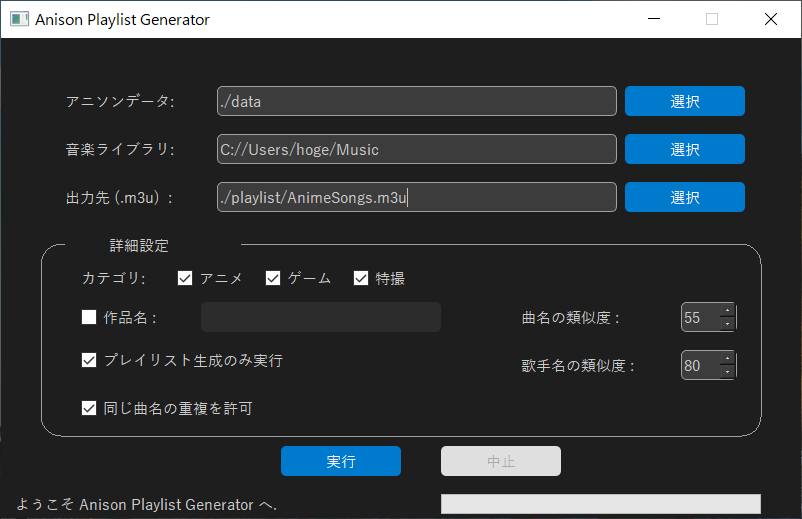
\includegraphics[width=0.95\hsize]{./figs/apg_ui.png}
    \caption{起動時の画面}
    \label{fig:apg_ui}
\end{figure}

\begin{itemize}
    \item アニソンデータ : AnisonGeneration様のデータが保存されているフォルダ.(変更非推奨)
    \item 音楽ライブラリ : 音楽ファイルが保存されているフォルダ.(初期値はc://Users/ユーザ名/Musicsです.)
    \item 出力先(.m3u) : 生成したプレイリストの保存先.必ず.m3uフォルダを指定してください.
    \item カテゴリ : アニメ,ゲーム,特撮カテゴリのデータを使用するかどうかを選択することができます.
    \item 作品名 : 特定のアニメだけのプレイリストを作成することができます.
    \item プレイリスト生成のみ実行 : 初回のみチェックを外してください.
    \item 同じ曲名の重複を許可 : チェックを入れると同じアーティスト内の同名の曲が含まれるようになります.
    \item 曲名の類似度 : 似たような名前の曲名もプレイリストに含めます.100に設定すると完全に一致した場合にプレイリストに含めます.
    \item 歌手名の類似度 : 似たような名前のアーティストもプレイリストに含めます.100に設定すると完全に一致した場合にプレイリストに含めます.
\end{itemize}

音楽ライブラリは音楽ファイルが保存されているフォルダのことです.
音楽ファイルを別の場所(例えばDドライブなど)に保存している場合は選択ボタンから適切なフォルダを選択してください.
選択が終わったら画面下部の実行を押してください.

\subsection{プレイリストの生成}
 プレイリストの実行を開始したら画面下部のプログレスバーが動き出します.プレイリスト生成の処理中は中止ボタン以外が押せなくなりますので,再度実行ボタンが押せるようになるまでお待ちください.
処理時間はパソコンに保存されている音楽ファイルの数に依存しますが,処理は数分で終わります.
\par また,初回実行時はinfo.dbというデータベースがapg.exeと同じフォルダ内に作成されます.2回目以降はデータベースを作成する必要はないので,プレイリスト生成のみ実行のチェックを外してプレイリストを作成してください.
なお,音楽ライブラリとアニソンデータのファイルに変更がある場合はプレイリスト生成のみ実行にチェックを入れて実行してください.


\section{注意点}
 本ソフトウェアは個人によって開発されたソフトウェアであり,正式なソフトウェア開発手法に則って開発が行われておりません.
バグは無くしたつもりですが,十分なテストが行えているとは言えない状態ですのでご注意ください.従って,本ソフトウェアの使用は自己責任でお願いいたします.
そのほかの仕様や注意点は次の通りです.

\subsection{対応するファイル形式}
 本ソフトウェアで扱うファイル形式は次の通りです.
\begin{itemize}
    \item 出力されるプレイリストファイルの形式 : m3u
    \item プレイリストに追加できる音楽ファイルの形式 : mp3, m4a, flac
\end{itemize}
\par 今後の開発で対応するファイル形式は増やす予定です.

\subsection{追加されるファイルについて}
 仕様上,アニソンではない音楽ファイルも.m3uファイルに追加されてしまう場合もあります.
例えば,CDから音楽を取り込んだときに曲名が
\begin{itemize}
    \item 曲名 (アルバムver.)
\end{itemize}
となっている場合があります.公開されているアニソンの情報は曲名だけですので,曲名が完全に一致したファイルだけプレイリストに追加しようとすると上記のファイルはプレイリストに追加されません.
そこで,公開されているアニソンの曲名と音楽ファイルの曲名の類似度を計算し,類似度が閾値よりも高ければ出力に追加という実装を行いました.
\par また,アニソンの歌手名は
\begin{itemize}
    \item アニメのキャラクター名 (cv. 声優名)
\end{itemize}
となっている場合があります.さらに複数のキャラクター名が歌手名となっている場合もあるため,タイトルと同様に類似度によるプレイリストの追加を採用しています.
(部分一致で検索をかければ良いとも思いましたが,実装上の都合で一度断念しました.)
\par 以上の理由から,プレイリスト作成時に曲が追加されない場合は,類似度の値を小さくして再度実行してください.
アニソンではない曲も追加されやすくなってしまいますが,その曲は手作業でプレイリストから削除していただければと思います.

\subsection{処理時間について}
 著者のパソコンに保存されている音楽ファイルの数は約8000件で,音楽ライブラリの登録に約1-2分,特に作品名を指定しなかった場合のプレイリスト生成に1分程度かかります.
数時間かかるようなことはありませんので,処理を停止して設定を見直してください.全体的な処理の高速化については今後の開発で改善予定です.

\subsection{不具合がや改善点を見つけた場合}
不具合や改善点などは著者のTwitterもしくはGithubまで.

\section*{謝辞}
\addcontentsline{toc}{section}{謝辞}
 アニソンの有益な情報を提供していただいているAnison Generation様に深くお礼申し上げます.

\section*{更新履歴}
\addcontentsline{toc}{section}{更新履歴}
\begin{itemize}
    \item Githubに公開 : 2020/01/22
    \item 説明書公開: 2020/03/04
\end{itemize}

\section*{リンク}
\addcontentsline{toc}{section}{リンク}
\begin{itemize}
    \item Anison Generation様 : http://anison.info/
    \item Twitter : https://twitter.com/10\_2rugata
    \item Github : https://github.com/temple1026/AnisonPlaylistGenerator
    \item Qiita : https://qiita.com/temple1026
\end{itemize}

\end{document}